%\documentclass[]{beamer}
\documentclass[handout]{beamer}\usepackage[]{graphicx}\usepackage[]{color}
%% maxwidth is the original width if it is less than linewidth
%% otherwise use linewidth (to make sure the graphics do not exceed the margin)
\makeatletter
\def\maxwidth{ %
  \ifdim\Gin@nat@width>\linewidth
    \linewidth
  \else
    \Gin@nat@width
  \fi
}
\makeatother

\definecolor{fgcolor}{rgb}{0.345, 0.345, 0.345}
\newcommand{\hlnum}[1]{\textcolor[rgb]{0.686,0.059,0.569}{#1}}%
\newcommand{\hlstr}[1]{\textcolor[rgb]{0.192,0.494,0.8}{#1}}%
\newcommand{\hlcom}[1]{\textcolor[rgb]{0.678,0.584,0.686}{\textit{#1}}}%
\newcommand{\hlopt}[1]{\textcolor[rgb]{0,0,0}{#1}}%
\newcommand{\hlstd}[1]{\textcolor[rgb]{0.345,0.345,0.345}{#1}}%
\newcommand{\hlkwa}[1]{\textcolor[rgb]{0.161,0.373,0.58}{\textbf{#1}}}%
\newcommand{\hlkwb}[1]{\textcolor[rgb]{0.69,0.353,0.396}{#1}}%
\newcommand{\hlkwc}[1]{\textcolor[rgb]{0.333,0.667,0.333}{#1}}%
\newcommand{\hlkwd}[1]{\textcolor[rgb]{0.737,0.353,0.396}{\textbf{#1}}}%
\let\hlipl\hlkwb

\usepackage{framed}
\makeatletter
\newenvironment{kframe}{%
 \def\at@end@of@kframe{}%
 \ifinner\ifhmode%
  \def\at@end@of@kframe{\end{minipage}}%
  \begin{minipage}{\columnwidth}%
 \fi\fi%
 \def\FrameCommand##1{\hskip\@totalleftmargin \hskip-\fboxsep
 \colorbox{shadecolor}{##1}\hskip-\fboxsep
     % There is no \\@totalrightmargin, so:
     \hskip-\linewidth \hskip-\@totalleftmargin \hskip\columnwidth}%
 \MakeFramed {\advance\hsize-\width
   \@totalleftmargin\z@ \linewidth\hsize
   \@setminipage}}%
 {\par\unskip\endMakeFramed%
 \at@end@of@kframe}
\makeatother

\definecolor{shadecolor}{rgb}{.97, .97, .97}
\definecolor{messagecolor}{rgb}{0, 0, 0}
\definecolor{warningcolor}{rgb}{1, 0, 1}
\definecolor{errorcolor}{rgb}{1, 0, 0}
\newenvironment{knitrout}{}{} % an empty environment to be redefined in TeX

\usepackage{alltt}
%\usepackage[dvips]{color}
%\usepackage{beamerprosper}
\usepackage{graphicx}
\usepackage{amsmath,amssymb,array,eucal}
\usepackage{xcolor}
\definecolor{beamer@blendedblue}{RGB}{86,155,189}
\definecolor{myblue}{RGB}{12,76,138}
\setbeamercolor{structure}{fg=myblue}
\definecolor{Ftitle}{RGB}{12,76,138}
\definecolor{Descitem}{RGB}{238,238,244}
\definecolor{StdTitle}{RGB}{12,76,138}
\definecolor{StdBody}{RGB}{213,24,0}
\definecolor{StdBody}{RGB}{213,24,0}

\definecolor{AlTitle}{RGB}{255, 190, 190}
\definecolor{AlBody}{RGB}{213,24,0}

\definecolor{ExTitle}{RGB}{201, 217, 217}
\definecolor{ExBody}{RGB}{213,24,0}

\setbeamercolor{frametitle}{fg = Ftitle}
\setbeamercolor{title}{fg = Ftitle}
\setbeamercolor{item}{fg = Ftitle}
\setbeamercolor{subitem}{fg = Ftitle}
\setbeamercolor{subsubitem}{fg = Ftitle}
\setbeamercolor{description item}{fg = myblue}
\setbeamercolor{titlelike}{fg=myblue}

%$Id: macros.tex,v 1.2 2006/02/13 14:23:55 rlw Exp rlw $
\newcommand{\Lmea}{{\cal L}} 
\newcommand{\scale}{\bflambda} 
\newcommand{\Scale}{\bfLambda} 
\newcommand{\bfscale}{\bflambda} 
\newcommand{\mean}{\bfchi}
\newcommand{\loc}{\bfchi}
\newcommand{\bfmean}{\bfchi}
\renewcommand{\k}{g}
\newcommand{\Gen}{{\cal G}}
\newcommand{\eps}{\epsilon}

\newcommand{\ind}{\mathrel{\mathop{\sim}\limits^{\mathit{ind}}}}
\newcommand{\iid}{\mathrel{\mathop{\sim}\limits^{\mathit{iid}}}}
\newcommand{\dis}{\mathrel{\mathop{=}\limits^{d}}}
\newcommand{\sgn}{\mathop{\rm sgn}}
\newcommand{\cmp}{h}
\newcommand{\dbdo}{d\beta ~ d\omega}
\newcommand{\real}{{\mathbb{R}}}
\newcommand{\Ber}{\mbox{\rm Ber}}
\newcommand{\GP}{\mbox{\rm GP}}
\newcommand{\SaS}{\text{S$\alpha$S}}
\newcommand{\RA}{{\real \times A}}
\newcommand{\RK}{{\real \times K}}
\newcommand{\RO}{{\real \times \Omega}} 
\newcommand{\RS}{{\bbR \times \LamS}}
  \newcommand{\set}[1]{\left\{#1\right\}}
  \newcommand{\bet}[1]{\left[#1\right]}
  \newcommand{\cet}[1]{\left(#1\right)}
%  \renewcommand{\half}{{\scriptstyle\frac12}}
\newcommand{\subA}{(\eps_1 < \beta \le \eps_2) \times \LamS}
 \newcommand{\uu}{{\big(\scale(x - \loc)\big)}}
 \newcommand{\uuj}{{\big(\scale_j(x-\loc_j)\big)}}
 \newcommand{\bbT}{{\mathbb{T}}}
 \newcommand{\ui}{{[0,1)}}
 \newcommand{\spq}[1]{\left|#1\right|^s_{pq}}
 \newcommand{\spqper}[1]{\left|#1\right|^{s\,*}_{pq}}
 \newcommand{\sspqper}[1]{\left\|#1\right\|^{s\,*}_{pq}}
 \newcommand{\sspq}[1]{\left\|#1\right\|^s_{pq}}    % Besov semi-norm
 \newcommand{\qp}[1]  {\left\|#1\right\|^q_p}         % Hilbert-space norm
 \newcommand{\qper}[1]{\left\|#1\right\|^{*\,q}_p}  % Periodic HS norm
 

\newcommand{\bbW}{{\mathbb{W}}}
\newcommand{\bbB}{{\mathbb{B}}}
\newcommand{\Sob}{{\ensuremath{\bbW^s_2}}}
\newcommand{\Besov}{{\ensuremath{\bbB^s_{pq}}}}
\newcommand{\Besper}{{\ensuremath{\bbB^{s\,*}_{pq}}}}
\newcommand{\Sobx}[1]{{\bbW^{#1}_2}}
\newcommand{\Besovx}[1]{{\bbB^{#1}_2}}
\newcommand{\SN}[1]{\|{#1}\|_\Sob}
% MATH LETTER DEFINITIONS
\newcommand{\Levy}{L{\'e}vy}
\newcommand{\nmathbf}{\bm}
\newcommand{\tabb}[1]{\hspace*{#1\parindent}}
%\newcommand{\G}{{g}}    % Really the same as \GB
\newcommand{\g}{{\phi}} %\newcommand{\g}{{g}}
\newcommand{\GB}{{g}}  
% Roman math Bold face 


\def\bfA{\nmathbf A}
\def\bfB{\nmathbf B}
\def\bfC{\nmathbf C}
\def\bfD{\nmathbf D}
\def\bfE{\nmathbf E}
\def\bfF{\nmathbf F}
\def\bfG{\nmathbf G}
\def\bfH{\nmathbf H}
\def\bfI{\nmathbf I}
\def\bfJ{\nmathbf J}
\def\bfK{\nmathbf K}
\def\bfL{\nmathbf L}
\def\bfM{\nmathbf M}
\def\bfN{\nmathbf N}
\def\bfO{\nmathbf O}
\def\bfP{\nmathbf P}
\def\bfQ{\nmathbf Q}
\def\bfR{\nmathbf R}
\def\bfS{\nmathbf S}
\def\bfT{\nmathbf T}
\def\bfU{\nmathbf U}
\def\bfV{\nmathbf V}
\def\bfW{\nmathbf W}
\def\bfX{\nmathbf X}
\def\bfY{\nmathbf Y}
\def\bfZ{\nmathbf Z}

\def\bfa{\nmathbf a}
\def\bfb{\nmathbf b}
\def\bfc{\nmathbf c}
\def\bfd{\nmathbf d}
\def\bfe{\nmathbf e}
\def\bff{\nmathbf f}
\def\bfg{\nmathbf g}
\def\bfh{\nmathbf h}
\def\bfi{\nmathbf i}
\def\bfj{\nmathbf j}
\def\bfk{\nmathbf k}
\def\bfl{\nmathbf l}
\def\bfm{\nmathbf m}
\def\bfn{\nmathbf n}
\def\bfo{\nmathbf o}
\def\bfp{\nmathbf p}
\def\bfq{\nmathbf q}
\def\bfr{\nmathbf r}
\def\bfs{\nmathbf s}
\def\bft{\nmathbf t}
\def\bfu{\nmathbf u}
\def\bfv{\nmathbf v}
\def\bfw{\nmathbf w}
\def\bfx{\nmathbf x}
\def\bfy{\nmathbf y}
\def\bfz{\nmathbf z}


\def\bfalpha  {\nmathbf \alpha}
\def\bfbeta   {\nmathbf \beta}
\def\bfgamma  {\nmathbf \gamma}
\def\bfdelta  {\nmathbf \delta}
\def\bfepsilon{\nmathbf \epsilon}
\def\bfvareps {\nmathbf \varepsilon}
\def\bfzeta   {\nmathbf \zeta}
\def\bfeta    {\nmathbf \eta}
\def\bftheta  {\nmathbf \theta}
\def\bfiota   {\nmathbf \iota}
\def\bfkappa  {\nmathbf \kappa}
\def\bflambda {\nmathbf \lambda}
\def\bfmu     {\nmathbf \mu}
\def\bfnu     {\nmathbf \nu}
\def\bfxi     {\nmathbf \xi}
\def\bfomicron{\nmathbf \omicron}
\def\bfpi     {\nmathbf \pi}
\def\bfrho    {\nmathbf \rho}
\def\bfsigma  {\nmathbf \sigma}
\def\bftau    {\nmathbf \tau}
\def\bfupsilon{\nmathbf \upsilon}
\def\bfphi    {\nmathbf \phi}
\def\bfpsi    {\nmathbf \psi}
\def\bfchi    {\nmathbf \chi}
\def\bfomega  {\nmathbf \omega}
\newcommand{\nubw}{{\tilde\nu}}  % no longer red!
\def\bfAlpha  {\nmathbf \Alpha}
\def\bfBeta   {\nmathbf \Beta}
\def\bfGamma  {\nmathbf \Gamma}
\def\bfDelta  {\nmathbf \Delta}
\def\bfEpsilon{\nmathbf \Epsilon}
\def\bfZeta   {\nmathbf \Zeta}
\def\bfEta    {\nmathbf \Eta}
\def\bfTheta  {\nmathbf \Theta}
\def\bfIota   {\nmathbf \Iota}
\def\bfKappa  {\nmathbf \Kappa}
\def\bfLambda {\nmathbf \Lambda}
\def\bfMu     {\nmathbf \Mu}
\def\bfNu     {\nmathbf \Nu}
\def\bfXi     {\nmathbf \Xi}
\def\bfOmicron{\nmathbf \Omicron}
\def\bfPi     {\nmathbf \Pi}
\def\bfRho    {\nmathbf \Rho}
\def\bfSigma  {\nmathbf \Sigma}
\def\bfTau    {\nmathbf \Tau}
\def\bfUpsilon{\nmathbf \Upsilon}
\def\bfPhi    {\nmathbf \Phi}
\def\bfPsi    {\nmathbf \Psi}
\def\bfChi    {\nmathbf \Chi}
\def\bfOmega  {\nmathbf \Omega}

% Number math Bold face

\newcommand{\bfzero}{{\nmathbf 0}}
\newcommand{\bfone}{{\nmathbf 1}}

% Estimators

\newcommand{\ttheta}{\tilde{\theta}}
\newcommand{\htheta}{\hat{\theta}}
\newcommand{\tbtheta}{\tilde{\bftheta}}
\newcommand{\hbtheta}{\hat{\bftheta}}
\newcommand{\tomega}{\tilde{\omega}}
\newcommand{\homega}{\hat{\omega}}
\newcommand{\tbomega}{\tilde{\bfomega}}
\newcommand{\hbomega}{\hat{\bfomega}}
\newcommand{\tlambda}{\tilde{\lambda}}
\newcommand{\hlambda}{\hat{\lambda}}
\newcommand{\tblambda}{\tilde{\bflambda}}
\newcommand{\hblambda}{\hat{\bflambda}}


% Calligraphic

\newcommand{\mc}[1]{\ensuremath{\mathcal{#1}}}

\newcommand{\cfA}{\mc{A}}
\newcommand{\cfB}{\mc{B}}
\newcommand{\cfC}{\mc{C}}
\newcommand{\cfD}{\mc{D}}
\newcommand{\cfE}{\mc{E}}
\newcommand{\cfF}{\mc{F}}
\newcommand{\cfG}{\mc{G}}
\newcommand{\cfH}{\mc{H}}
\newcommand{\cfI}{\mc{I}}
\newcommand{\cfJ}{\mc{J}}
\newcommand{\cfK}{\mc{K}}
\newcommand{\cfL}{\mc{L}}
\newcommand{\cfM}{\mc{M}}
\newcommand{\cfN}{\mc{N}}
\newcommand{\cfO}{\mc{O}}
\newcommand{\cfP}{\mc{P}}
\newcommand{\cfQ}{\mc{Q}}
\newcommand{\cfR}{\mc{R}}
\newcommand{\cfS}{\mc{S}}
\newcommand{\cfT}{\mc{T}}
\newcommand{\cfU}{\mc{U}}
\newcommand{\cfV}{\mc{V}}
\newcommand{\cfX}{\mc{X}}
\newcommand{\cfY}{\mc{Y}}
\newcommand{\cfZ}{\mc{Z}}

\newcommand{\bmc}[1]{\ensuremath{\boldsymbol{\mathcal{#1}}}}

\newcommand{\bcfA}{\bmc{A}}
\newcommand{\bcfB}{\bmc{B}}
\newcommand{\bcfC}{\bmc{C}}
\newcommand{\bcfD}{\bmc{D}}
\newcommand{\bcfE}{\bmc{E}}
\newcommand{\bcfF}{\bmc{F}}
\newcommand{\bcfG}{\bmc{G}}
\newcommand{\bcfH}{\bmc{H}}
\newcommand{\bcfI}{\bmc{I}}
\newcommand{\bcfJ}{\bmc{J}}
\newcommand{\bcfK}{\bmc{K}}
\newcommand{\bcfL}{\bmc{L}}
\newcommand{\bcfM}{\bmc{M}}
\newcommand{\bcfN}{\bmc{N}}
\newcommand{\bcfO}{\bmc{O}}
\newcommand{\bcfP}{\bmc{P}}
\newcommand{\bcfQ}{\bmc{Q}}
\newcommand{\bcfR}{\bmc{R}}
\newcommand{\bcfS}{\bmc{S}}
\newcommand{\bcfT}{\bmc{T}}
\newcommand{\bcfU}{\bmc{U}}
\newcommand{\bcfV}{\bmc{V}}
\newcommand{\bcfW}{\bmc{W}}
\newcommand{\bcfX}{\bmc{X}}
\newcommand{\bcfY}{\bmc{Y}}
\newcommand{\bcfZ}{\bmc{Z}}

% Special symbols

\newcommand{\reals}{\mbox{\rm I\kern-.20em R}}
\newcommand{\sreals}{\mbox{\small \rm I\kern-.20em R}}
\newcommand{\LamS}{{\cS^d_+}}

% MATHEMATICAL NOTATION

% Operators

\newcommand{\bg}{\;\bigg\vert\;}
\newcommand{\pr}{\mbox{\rm Pr}}
\newcommand{\D}{\mbox{\rm D}}
\newcommand{\E}{\mbox{\rm E}}
\newcommand{\Mo}{\mbox{\rm Mo}}
\newcommand{\Me}{\mbox{\rm Me}}
\newcommand{\Cov}{\mbox{\rm Cov}}
\newcommand{\Var}{\mbox{\rm Var}}
\newcommand{\Corr}{\mbox{\rm Corr}}
\newcommand{\Q}{\mbox{\rm Q}}

% Distributions
\newcommand{\BeBi}{\mbox{\rm BeBi}}
\newcommand{\Be}{\mbox{\rm Be}}
\newcommand{\Bi}{\mbox{\rm Bi}}
\newcommand{\Br}{\mbox{\rm Br}}
\newcommand{\Ca}{\mbox{\rm Ca}}
\newcommand{\Di}{\mbox{\rm Di}}
\newcommand{\Ex}{\mbox{\rm Ex}}
\newcommand{\Fs}{\mbox{\rm Fs}}
\newcommand{\Ga}{\mbox{\sf G}}
\newcommand{\Ge}{\mbox{\rm Ge}}
\newcommand{\GaGa}{\mbox{\rm GaGa}}
\newcommand{\Hy}{\mbox{\rm Hy}}
\newcommand{\IGa}{\mbox{\rm IGa}}
\newcommand{\IPa}{\mbox{\rm IPa}}
\newcommand{\Lo}{\mbox{\rm Lo}}
\newcommand{\Mu}{\mbox{\rm Mu}}
\newcommand{\N}{\mbox{\rm N}}
\newcommand{\NBi}{\mbox{\rm NBi}}
\newcommand{\NGa}{\mbox{\rm NGa}}
\newcommand{\NWi}{\mbox{\rm NWi}}
\newcommand{\Pa}{\mbox{\rm Pa}}
\newcommand{\Po}{\mbox{\sf P}}
\newcommand{\PoGa}{\mbox{\rm PoGa}}
\newcommand{\Ra}{\mbox{\rm Ra}}
\newcommand{\REx}{\mbox{\rm REx}}
\newcommand{\St}{\mbox{\rm St}}
\newcommand{\Un}{\mbox{\rm Un}}
\newcommand{\Wi}{\mbox{\rm Wi}}

% General Mathematics

\newcommand{\dd}[1]{\,d{#1}}
\newcommand{\barx}{\ensuremath{\bar{x}}}
\newcommand{\comb}[2]{{#1\choose#2}}
\newcommand{\ontop}[2]{{#1\atop#2}}
\newcommand{\h}{{\small\ensuremath{1\over2}}}
\newcommand{\hh}[2]{{\small\ensuremath{#1\over#2}}}

\newcommand{\fn}[1]{\hbox{\textrm{#1}}}
\newcommand{\cred}{\fn{Cr}}
\newcommand\dlim{\mathop{\rm \hbox{$\delta$}lim}}
\newcommand{\goto}{\rightarrow}
\newcommand{\gotoinf}{\rightarrow \infty}

\newcommand{\data}{\ensuremath{\bfx=\{x_1,\ldots,x_n\}}}
\newcommand{\brow}[2]{\ensuremath{\{{#1}_1,\ldots,{#1}_{#2}\}}}
\newcommand{\prow}[2]{\ensuremath{({#1}_1,\ldots,{#1}_{#2})}}

\newcommand{\met}{\thinspace{\rm m}}\newcommand{\km}{\thinspace{\rm km}}
\newcommand{\xbar}{\overline X}%
\newcommand{\xbbar}{\overline{\overline X}}%
\font\ss=cmss12
 \newcommand{\OFP}{(\Omega,\cF,\P)}
 \newcommand{\bbC}{\mathbb{C}}
 \newcommand{\bbF}{\mathbb{F}}
 \newcommand{\bbN}{\mathbb{N}}
 \newcommand{\bbR}{\mathbb{R}}
 \newcommand{\bbX}{\mathbb{X}}
 \newcommand{\bbZ}{\mathbb{Z}}
 \newcommand{\one}[1]{\mathbf{1}_{\{#1\}}}
 \newcommand{\cA}{{\cal A}}
 \newcommand{\cB}{{\cal B}} 
 \newcommand{\cE}{{\cal E}}
 \newcommand{\cF}{{\cal F}}
 \newcommand{\cG}{{\cal G}}
 \newcommand{\cH}{{\cal H}}
 \newcommand{\cM}{{\cal M}}
 \newcommand{\cR}{{\cal R}}
 \newcommand{\cS}{{\cal S}}
 \newcommand{\cT}{{\cal T}}
 \newcommand{\cX}{{\cal X}}
 \newcommand{\cY}{{\cal Y}}
 \newcommand{\cZ}{{\cal Z}}
 \newcommand{\eF}{{\CMcal F}}
 \newcommand{\eG}{{\CMcal G}} 
 \newcommand{\eH}{{\CMcal H}}
 \renewcommand{\P}{{\sf{P}}} 
 \renewcommand{\E}{{\sf{E}}}
 \newcommand{\Ev}{{\sf{Ev}}}%
 \newcommand{\V}{{\sf{V}}} 
 \renewcommand{\Cov}{{\sf{Cov}}}
 %\newcommand{\Be}{\textsf{Be}}
 %\newcommand{\Bi}{\textsf{Bi}}
 %\newcommand{\Ex}{\textsf{Ex}}\newcommand{\Ga}{\textsf{Ga}}
 %\newcommand{\Di}{\textsf{Di}}\newcommand{\Ge}{\textsf{Ge}}
 %\newcommand{\IG}{\textsf{IG}}\newcommand{\Lv}{\textsf{Lv}}
 %\newcommand{\HG}{\textsf{HG}}\newcommand{\MN}{\textsf{MN}}
\newcommand{\NB}{\textsf{NB}}\newcommand{\No}{\textsf{N}}
\newcommand{\LN}{\textsf{LN}}
\newcommand{\Lv}{\mbox{\rm Lv}}
%\newcommand{\Pa}{\textsf{Pa}}
% \newcommand{\Po}{\textsf{Po}}\newcommand{\Un}{\textsf{Un}}
 \newcommand{\argmax}{\textrm{argmax}}
 \renewcommand{\th}{{\ensuremath^{\mbox{\tiny th}}}}
 \newcommand{\nd}{{\ensuremath^{\mbox{\tiny nd}}}}
 \newcommand{\st}{{\ensuremath^{\mbox{\tiny st}}}}
 \newcommand{\ii}{{\ensuremath{\bar{i}}}}% \newcommand{\ii}{{\hat i}}
 \newcommand{\jj}{{\ensuremath{\bar{j}}}}%
 \newcommand{\R}{\texttt{R}}
 \newcommand{\mayeq}{\mathrel{\mathop{=}\limits^?}}
 \newcommand{\pperp}{\mathrel{{\rlap{$~\perp$}\perp\,\,}}}
 \newbox\asbox
 \setbox\asbox=\hbox{\vrule height 15pt depth3.5pt width0pt}
 \def\astrut{\relax\ifmmode\copy\strutbox\else\unhcopy\strutbox\fi}
 \def\Strut{\vrule width0pt height 16pt depth 4pt}%
%\font\tinyss=cmss8 at 8truept % for ^T etc
\newcommand{\tsf}[1]{\textsf{\tiny{#1}}}
\newcommand{\fxa}{\mbox{$f(x\mid\alpha)$}}
\newcommand{\fxt}{\mbox{$f(x\mid\theta)$}}
\newcommand{\fxat}{\mbox{$f(x\mid\alpha,\theta)$}}
\newcommand{\tp}{^{\tsf{T}}}
\newcommand{\as}{\textit{a.s.}}
\newcommand{\ie}{\textit{i.e.{}}}
\newcommand{\etc}{\textit{etc}}
\newcommand{\eg}{\textit{e.g.{}}}%
\newcommand{\half}{{\frac12}}
\newcommand{\Sec}[1]{Section\thinspace(\ref{#1})}
\newcommand{\Thm}[1]{Theorem\thinspace\ref{#1}}
\newcommand{\Cor}[1]{Corollary\thinspace\ref{#1}}
\newcommand{\Eqn}[1]{Equation\thinspace(\ref{#1})}
\newcommand{\Fig}[1]{Figure\thinspace(\ref{#1})}
\newcommand{\Figs}[2]{Figures\thinspace(\ref{#1}) and (\ref{#2})}
\newcommand{\Figab}[2]{Figure\thinspace(\ref{#1}#2)}
\newcommand{\Tab}[1]{Table\thinspace(\ref{#1})}
\newcommand{\jth}{{\ensuremath j^{\mbox{\tiny th}}}}%
\providecommand{\ij}{_{ij}} \newcommand{\ji}[1]{_{ij#1}}%
\newcount\ola \newcount\olb \newcount\olc \newcount\old \newcount\ole
\newcount\och\newcount\level
\newtheorem{cor}{Corollary}
\newtheorem{define}{Definition}
\newtheorem{lem}{Lemma}
\newtheorem{prob}{Problem}
\newtheorem{prop}{Proposition}
\newtheorem{thm}{Theorem}
\def\OL#1{\par\noindent\hangindent=#1\parindent % Outline
  \kern1\hangindent\ignorespaces}%
\def\ol#1{%
    \level=#1
    \ifcase\level
    \ola=0 \olb=0 \olc=0 \old=0 \ole=0\or         % Level 0 (reset)
    \olb=0 \olc=0 \old=0 \ole=0 \advance\ola by 1 % Level 1
    \gdef\olev{\uppercase\expandafter{\romannumeral\ola}} \or
    \olc=0 \old=0 \ole=0 \advance\olb by 1        % Level 2
    \och=64 \advance\och by\olb
    \gdef\olev{\char\och}\or
    \old=0 \ole=0 \advance\olc by 1               % Level 3
    \och=48 \advance\och by\olc
    \gdef\olev{\char\och}\or
    \ole=0 \advance\old by 1                      % Level 4
    \och=96 \advance\och by\old
    \gdef\olev{\char\och}\or
    \advance\ole by 1                             % Level 5
    \gdef\olev{\romannumeral\ole} \or
    \message{Outline depth too deep: #1}\fi
    \ifnum\level>0 \OL\level\llap{\olev.\enspace}\ignorespaces\fi}%
\long\def\comment#1/*#2*/{\endcomment}%
\def\endcomment{\relax}%
%
\makeatletter % Find hours (count1) and minutes (count2) past midnight:
\count1\time \divide\count1 60 \count2=-\count1
\multiply\count2 60 \advance\count2 \time
\edef\now{\two@digits{\the\count1}:\two@digits{\the\count2}}
%\renewcommand\section{\@startsection     % Smaller and sans-serif
%    {section}{1}{\z@}{-3.5ex \@plus -1ex \@minus -.2ex}%
%    {2.3ex \@plus.2ex}{\normalfont\large\bfseries\sffamily}}
%\renewcommand\subsection{\@startsection
%    {subsection}{2}{\z@}{-3.25ex\@plus -1ex \@minus -.2ex}%
%    {1.5ex \@plus .2ex}{\normalfont\large\bfseries\sffamily}}
%\renewcommand\subsubsection{\@startsection
%    {subsubsection}{3}{\z@}{-3.25ex\@plus -1ex \@minus -.2ex}%
%    {1.5ex \@plus .2ex}{\normalfont\normalsize\bfseries\sffamily}}
%\def\@seccntformat#1{\csname the#1\endcsname.\quad} % Add . to sec num's
%\long\def\@makecaption#1#2{%                          Use . not : in cap'ns
%  \vskip\abovecaptionskip
%  \sbox\@tempboxa{#1. #2}%
%  \ifdim \wd\@tempboxa >\hsize
%    #1. #2\par
%  \else
%    \global \@minipagefalse
%    \hb@xt@\hsize{\hfil\box\@tempboxa\hfil}%
%  \fi
%  \vskip\belowcaptionskip}
% BEAMER FIX START
\def\newblock{\beamer@newblock}
% BEAMER FIX END
\makeatother

\def\wbox#1#2#3{{\vcenter{\vbox{\hrule height.#3pt
    \hbox{\vrule width.#3pt height#1pt \kern#2pt \vrule width.#3pt}%
                            \hrule height.#3pt}}}}%
\def\Proof.{\medbreak\noindent{\bf Proof.\enspace}}
\def\qed{{\nobreak\hfill\penalty0\hbox to1truecm{}\nobreak
    \hfill$\wbox634$\par\bigskip}}%

\usepackage{verbatim}

\def\logit{\textsf{logit}}
\def\SE{\textsf{SE}}
\def\C{\textsf{CAGE}}
\def\L{\textsf{LIGHT}}
\def\Li{\textsf{LITTER}}
\def\G{\textsf{GAP}}
\def\S{\textsf{SURV}}
\def\V{\textsf{SPECIES}}


\title{Binary Regression}

\author{GH Chapter 5, ISL Chapter 4 }
\date{\today}
\IfFileExists{upquote.sty}{\usepackage{upquote}}{}
\begin{document}
\maketitle



\begin{frame}[fragile]\frametitle{Seedling Survival}

  Tropical rain forests have up to 300 species of trees per hectare,
  which leads to difficulties when studying processes which occur at
  the community level. To gain insight into species responses, a
  sample of seeds were selected from a suite of eight species selected
  to represent the range of regeneration types which occur in this
  community.
\begin{verbatim}
Name       Size Cotyledon type
Ardisia       3 H
C. biflora    7 H
Gouania       1 E      Size = 1 smallest to 8 largest
Hirtella      8 H      E = Epigeal  - cotyledons
Inga          4 H      H = Hypogeal - seed food reserves
Maclura       2 E
C. racemosa   6 H
Strychnos     5 E
\end{verbatim}
%Epigeal species rely on the cotyledons for
%photosynthesis and production of energy to become estabished. Seed
%size tends to be small, with little reserves in the seeds. Hypogeal
%species tend to have larger seeds, and can rely on reserves in the
%seed to produce energy, thus if initial leaves are lost to predators,
%there may still be additional reserves that can be used to produce
%additional leaves. Larger seeds, however, may be easier to spot by
%predators.
\end{frame}

\begin{frame}\frametitle{Experimental Design}
 This representative community was then placed in
  experimental plots manipulated to mimic natural conditions \pause
  \begin{itemize}
  \item 8 PLOTs: 4 in forest gaps, 4 in understory conditions \pause
  \item Each plot split in half:  mammals were excluded from
  one half with a CAGE \pause
  \item 4 subplots within each CAGE/NO CAGE \pause
  \item 6 seeds of each SPECIES plotted in each SUBPLT \pause
  \item 4 LITTER levels applied to each SUBPLT \pause
  \item LIGHT levels at forest floor recorded \pause
  \item  SURV  an indicator of whether they germinated and survived was
  recorded \pause
  \end{itemize}
  Which variables are important in determining whether a
  seedling will survive? Are there interactions that influence
  survival probabilities?
\end{frame}

\begin{frame}\frametitle{Modeling Survival}
Distribution for Survival of a single Seedling is a Bernoulli random variable
$$  \E[\S_i \mid {\textsf covariates} ] = \pi_i $$ \pause

How should we relate covariates to probability of survival? \pause

For example, probability of survival may depend on whether there was a
\C\ to prevent animals from eating the seedling or \L\ levels. \pause
\begin{itemize}
\item Naive approach: Regress \S\ on \C\ and \L\
$$\hat{\pi}_i = \hat{\beta}_0 + \hat{\beta}_1 \C_i + \hat{\beta}_2 \L_i$$ \pause
\item Problems:
  \begin{itemize}
  \item  Fitted values of probabilities are not constrained to
  (0, 1) \pause
  \item Variances are not constant $\pi_i(1 - \pi_i)$ under Bernoulli model \pause
 \end{itemize}
\item Unbiased? \pause
\end{itemize}
\end{frame}

\begin{frame}[fragile]\frametitle{plot of SURV \& CAGE }

\begin{knitrout}
\definecolor{shadecolor}{rgb}{0.969, 0.969, 0.969}\color{fgcolor}\begin{kframe}
\begin{alltt}
\hlstd{seeds} \hlkwb{=} \hlkwd{read.table}\hlstd{(}\hlstr{"seeds.txt"}\hlstd{,} \hlkwc{header}\hlstd{=}\hlnum{TRUE}\hlstd{)}
\hlkwd{mosaicplot}\hlstd{(SURV} \hlopt{~} \hlstd{CAGE,} \hlkwc{data}\hlstd{=seeds)}
\end{alltt}
\end{kframe}
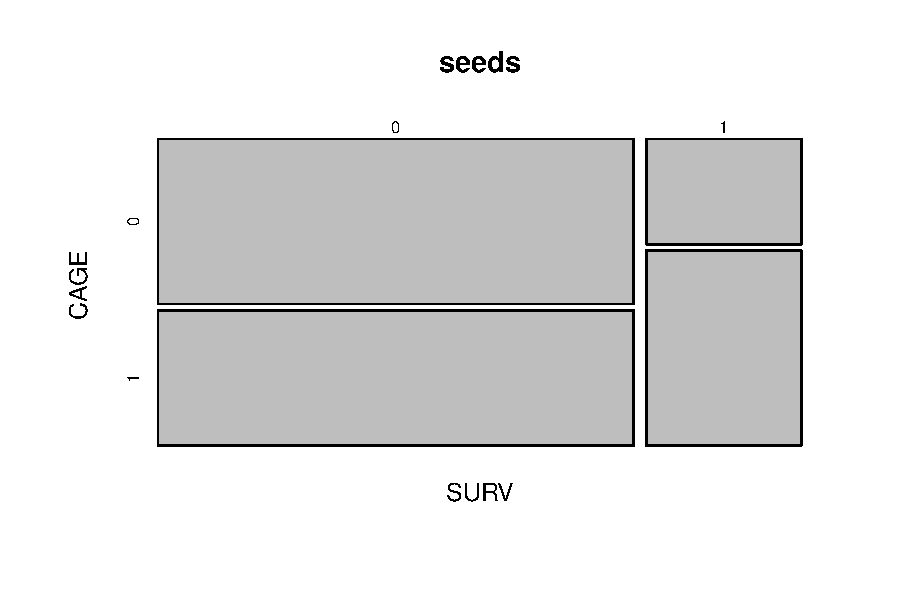
\includegraphics[width=\maxwidth]{figure/unnamed-chunk-2-1} 

\end{knitrout}
\end{frame}

\begin{frame}[fragile]\frametitle{plot of SURV versus LIGHT and CAGE }

\begin{knitrout}
\definecolor{shadecolor}{rgb}{0.969, 0.969, 0.969}\color{fgcolor}
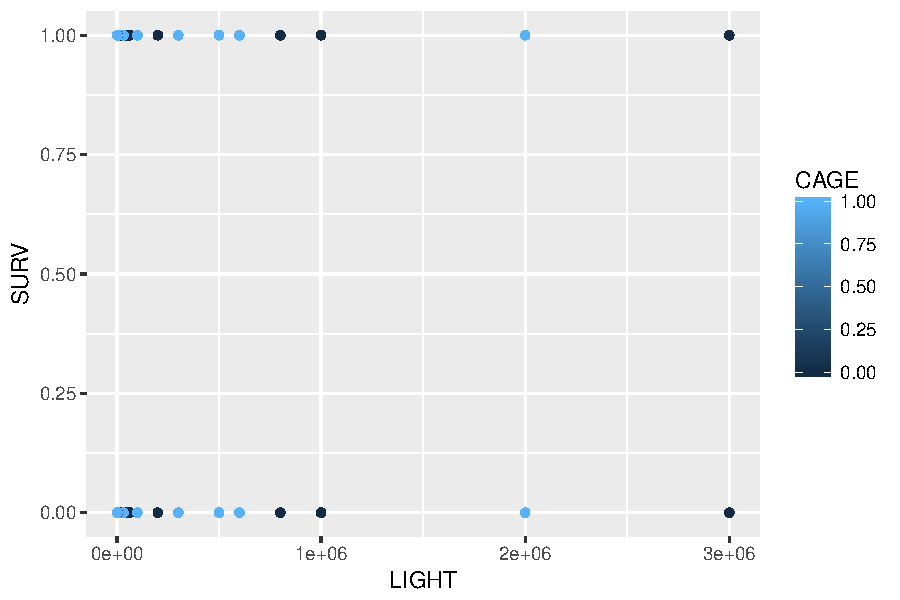
\includegraphics[width=\maxwidth]{figure/unnamed-chunk-3-1} 

\end{knitrout}
\end{frame}

\begin{frame}[fragile]\frametitle{plot of SURV versus LIGHT and CAGE jittered}

\begin{knitrout}
\definecolor{shadecolor}{rgb}{0.969, 0.969, 0.969}\color{fgcolor}
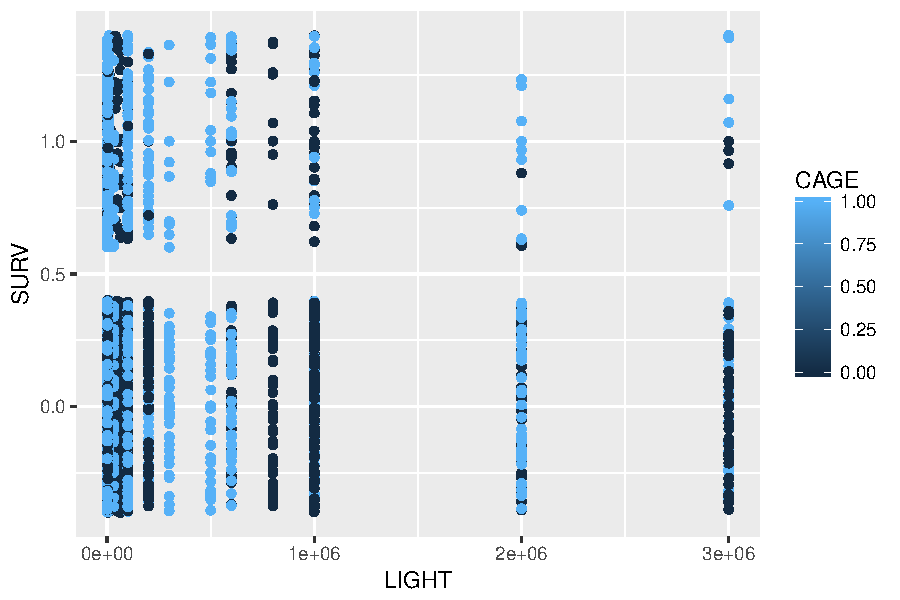
\includegraphics[width=\maxwidth]{figure/unnamed-chunk-4-1} 

\end{knitrout}
\end{frame}


\begin{frame}\frametitle{Logistic Regression}
To build in the necessary constraints that the probabilities are
between 0 and 1 convert to log-odds or ``logits'' \pause
\begin{itemize}
\item Odds of survival: $\pi_i/(1 - \pi_1)$ \pause
$$ \logit(\pi_i) \stackrel{\sf def}{=} \log\left(\frac {\pi_i} {1 -
    \pi_i} \right) = \beta_0 + \beta_1 \C_i + \beta_2 \L_i = \eta_i$$ \pause
\item $\eta_i$ is the linear predictor \pause
\item \logit\  is the {\it link} function that relates the mean $\pi_i$
  to the linear predictor $\eta_i$ \pause
\item Generalized Linear Models (GLMs) \pause
\item Find Maximum Likelihood Estimates (optimization problem)
\end{itemize}
\end{frame}


\begin{frame}\frametitle{Logits}
To convert from the linear predictor $\eta$ to the mean $\pi$,
  use the inverse transformation: \pause
  \begin{itemize}
\item log odds (\S = 1) = $\eta$ \pause
\item odds $(\S = 1) = \exp(\eta) = \omega$ \pause
\item $\pi$ = odds/(1 + odds) = $\omega/(1 + \omega)$ \pause
\item $\omega = \pi/(1 - \pi)$ \pause
  \end{itemize}
Can go in either direction
\end{frame}

\begin{frame}\frametitle{Interpretation of Coefficients}
$$\omega_i = \exp(\beta_0 + \beta_1 \C_i + \beta_2 \L_i)$$ \pause
\begin{itemize}
\item When all explanatory variables are 0 (\C = 0, \L = 0), the odds
  of survival are $\exp(\beta_0)$ \pause
\item The ratio of odds (or odds ratio) at $X_j = A$ to odds at $X_j =
  B$, for fixed values of the other explanatory variables is
  \begin{align*}
   \textsf{ Odds ratio} &= \frac{\omega_A}{\omega_b}  = \exp(\beta_j
   (A - B)) \\  \pause
 \textsf{ Odds ratio} &= \frac{\omega_A}{\omega_b}  = \exp(\beta_j)
   \text{ if } A - B = 1\\ \pause
\textsf{Odds}(X_j = A) &= \exp(\beta_j) \cdot \textsf{Odds}(X_j = B)
  \end{align*}
\item Coefficients are log odds ratios \pause
\end{itemize}
\end{frame}


\begin{frame}[fragile]\frametitle{R Code}
  \begin{itemize}
  \item use {\tt glm()} rather than {\tt lm()} \pause
  \item model formula as before  \pause
  \item need to specify family (and link if not default) \pause
  \end{itemize}
\begin{knitrout}
\definecolor{shadecolor}{rgb}{0.969, 0.969, 0.969}\color{fgcolor}\begin{kframe}
\begin{alltt}
\hlstd{seeds} \hlkwb{=} \hlkwd{read.table}\hlstd{(}\hlstr{"seeds.txt"}\hlstd{,} \hlkwc{header}\hlstd{=}\hlnum{TRUE}\hlstd{)}
\hlstd{seeds.glm0} \hlkwb{=} \hlkwd{glm}\hlstd{(SURV} \hlopt{~} \hlnum{1}\hlstd{,} \hlkwc{data}\hlstd{=seeds,} \hlkwc{family}\hlstd{=binomial)}
\hlstd{seeds.glm1} \hlkwb{=} \hlkwd{glm}\hlstd{(SURV} \hlopt{~}  \hlstd{CAGE} \hlopt{+} \hlstd{LIGHT,}
                 \hlkwc{family} \hlstd{= binomial,}
                 \hlkwc{data}\hlstd{=seeds)}
\end{alltt}
\end{kframe}
\end{knitrout}
\end{frame}


\begin{frame}[fragile]\frametitle{Estimates}

\begin{kframe}
\begin{alltt}
\hlkwd{library}\hlstd{(xtable)}
\hlkwd{xtable}\hlstd{(}\hlkwd{summary}\hlstd{(seeds.glm1)}\hlopt{$}\hlstd{coef,}
       \hlkwc{digits}\hlstd{=}\hlkwd{c}\hlstd{(}\hlnum{0}\hlstd{,} \hlnum{4}\hlstd{,} \hlnum{4}\hlstd{,} \hlnum{1}\hlstd{,}\hlopt{-}\hlnum{2}\hlstd{))}
\end{alltt}
\end{kframe}% latex table generated in R 3.3.2 by xtable 1.8-2 package
% Tue Jan 31 22:43:50 2017
\begin{table}[ht]
\centering
\begin{tabular}{rrrrr}
  \hline
 & Estimate & Std. Error & z value & Pr($>$$|$z$|$) \\ 
  \hline
(Intercept) & -1.4373 & 0.0709 & -20.3 & 3.02E-91 \\ 
  CAGE & 0.7858 & 0.0875 & 9.0 & 2.79E-19 \\ 
  LIGHT & -0.0000 & 0.0000 & -5.3 & 9.09E-08 \\ 
   \hline
\end{tabular}
\end{table}


  \begin{itemize}
  \item Coefficient for the dummy variable \C = 0.79 \pause
  \item If \C\ increases by 1 unit (No \C\ to \C) the odds of survival change by
  $\exp(.79) = 2.2$ \pause
\item The odds of survival in a \C\ are 2.2 times higher than odds of
  survival in the open. \pause
  \end{itemize}
\end{frame}


\begin{frame}[fragile]\frametitle{Confidence Intervals}


  \begin{itemize}
  \item MLEs are approximately normally distributed (large samples) \pause
    \begin{itemize}
    \item mean $\beta_j$ \pause
    \item estimated variance $\SE(\beta_j)^2$ \pause
    \end{itemize}
\item Asymptotic posterior distribution for $\beta_j$ is
  $N(\hat{\beta}_j, \SE(\beta_j)^2)$ \pause
\item $(1 - \alpha) 100\%$ CI based on normal theory:
$$ \hat{\beta}_j \pm Z_{\alpha/2} \SE(\beta_j)$$ \pause
\item $95\%$ CI for coefficient for \C:

$$  0.7858\pm 1.96 * 0.7858 = (0.62, 0.96) $$ \pause
\item Exponentiate to obtain interval for odds ratio:
$\exp(0.62), \exp(0.96) = (1.85, 2.607)$ \pause
  \end{itemize}
 The odds of survival in a \C\  are 1.85 to 2.607 times higher than odds of  survival in the open (with confidence  $0.95)$.
\end{frame}


\begin{frame}[fragile]\frametitle{Deviance}
The concept of Deviance replaces Sum-of-Squares in GLMs \pause
\begin{itemize}
\item residual deviance = -2 log likelihood at MLEs \pause
$$ -2 \sum_i y_i\log(\hat{\pi}_i) + (1 - y_i)\log(1 - \hat{\pi}_i)$$
$$\log(\hat{\pi}_i/(1 - \hat{\pi}_i)) = \hat{\beta}_0 + \C\ \hat{\beta}_1 + \L\ \hat{\beta}_2$$
\item null deviance = residual deviance under model with constant mean (Total
  Sum of Squares in Gaussian) \pause
\item analysis of deviance \pause
\item change in (residual) deviance has an asymptotic $\chi^2$
  distribution with degrees of freedom based on the change in
  number of parameters  \pause
\end{itemize}
\end{frame}

\begin{frame}[fragile]\frametitle{Analysis of Deviance Table}

\begin{knitrout}
\definecolor{shadecolor}{rgb}{0.969, 0.969, 0.969}\color{fgcolor}\begin{kframe}
\begin{alltt}
\hlkwd{anova}\hlstd{(seeds.glm0, seeds.glm1,} \hlkwc{test}\hlstd{=}\hlstr{"Chi"}\hlstd{)}
\end{alltt}
\begin{verbatim}
## Analysis of Deviance Table
## 
## Model 1: SURV ~ 1
## Model 2: SURV ~ CAGE + LIGHT
##   Resid. Df Resid. Dev Df Deviance  Pr(>Chi)    
## 1      3071     3426.1                          
## 2      3069     3299.0  2   127.09 < 2.2e-16 ***
## ---
## Signif. codes:  0 '***' 0.001 '**' 0.01 '*' 0.05 '.' 0.1 ' ' 1
\end{verbatim}
\end{kframe}
\end{knitrout}

OverDispersion/Lack of Fit?
\end{frame}

\begin{frame}[fragile]\frametitle{Lack of Fit}

\begin{itemize}
\item Lack of fit if residual deviance larger than expected
\item no variance needed to compare
\item Residual Deviance has a $\chi^2$ with $n - p$ df
\item p-value = $P(\chi^2_{n-p} > \text{ observed deviance})$
\end{itemize}
\begin{knitrout}
\definecolor{shadecolor}{rgb}{0.969, 0.969, 0.969}\color{fgcolor}\begin{kframe}
\begin{alltt}
\hlkwd{pchisq}\hlstd{(seeds.glm1}\hlopt{$}\hlstd{deviance, seeds.glm1}\hlopt{$}\hlstd{df.residual,}
       \hlkwc{lower}\hlstd{=}\hlnum{FALSE}\hlstd{)}
\end{alltt}
\begin{verbatim}
## [1] 0.002024634
\end{verbatim}
\end{kframe}
\end{knitrout}

Surprising result if model were true.

\end{frame}

\begin{frame}[fragile]\frametitle{Diagnostic Plots: { plot(seeds.glm1)}}
\begin{knitrout}
\definecolor{shadecolor}{rgb}{0.969, 0.969, 0.969}\color{fgcolor}
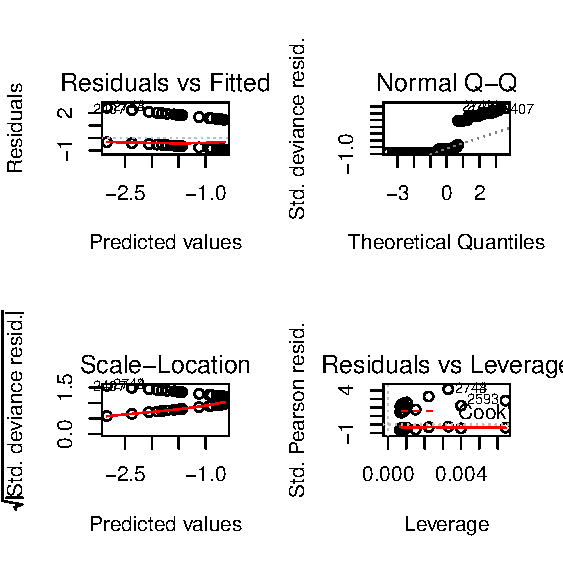
\includegraphics[width=\maxwidth]{figure/unnamed-chunk-7-1} 

\end{knitrout}


\end{frame}

\begin{frame}[fragile]\frametitle{termplot}

\begin{knitrout}
\definecolor{shadecolor}{rgb}{0.969, 0.969, 0.969}\color{fgcolor}\begin{kframe}
\begin{alltt}
\hlkwd{termplot}\hlstd{(seeds.glm1,} \hlkwc{term}\hlstd{=}\hlstr{'LIGHT'}\hlstd{,} \hlkwc{rug}\hlstd{=T)}
\end{alltt}
\end{kframe}
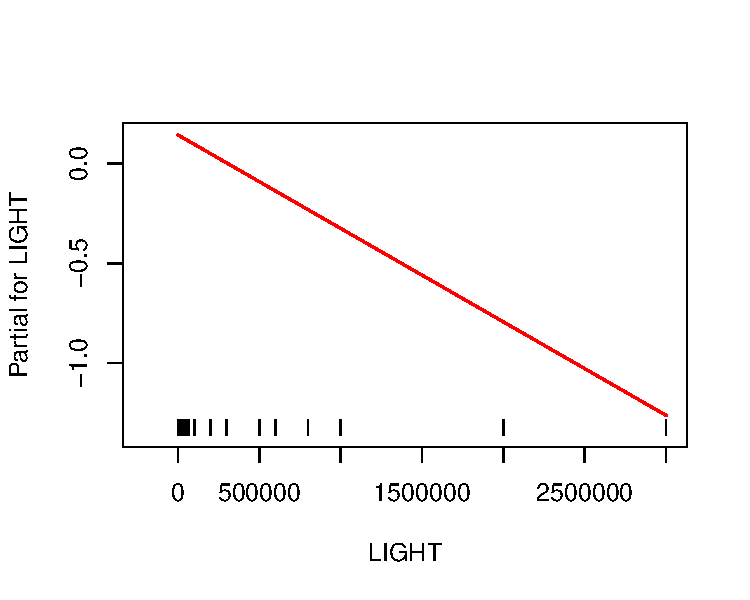
\includegraphics[width=\maxwidth]{figure/termplot-1} 

\end{knitrout}

see \url{http://www.clayford.net/statistics/tag/termplot/}
\end{frame}

\begin{frame}[fragile]\frametitle{log(LIGHT)}
\begin{knitrout}
\definecolor{shadecolor}{rgb}{0.969, 0.969, 0.969}\color{fgcolor}\begin{kframe}
\begin{alltt}
\hlstd{seeds.glm2} \hlkwb{=} \hlkwd{glm}\hlstd{(SURV} \hlopt{~}  \hlstd{CAGE} \hlopt{+} \hlkwd{log}\hlstd{(LIGHT),}
                 \hlkwc{family} \hlstd{= binomial,}
                 \hlkwc{data}\hlstd{=seeds)}
\hlkwd{termplot}\hlstd{(seeds.glm2,} \hlkwc{term}\hlstd{=}\hlstr{"log(LIGHT)"}\hlstd{,} \hlkwc{rug}\hlstd{=T)}
\end{alltt}
\end{kframe}
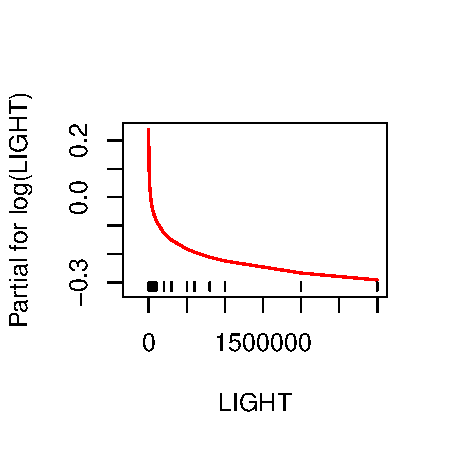
\includegraphics[width=\maxwidth]{figure/seeds_glm2-1} 

\end{knitrout}

\end{frame}
\begin{frame}[fragile]\frametitle{Other Variables}
\begin{small}
\begin{kframe}
\begin{alltt}
\hlstd{seeds.glm3} \hlkwb{=} \hlkwd{glm}\hlstd{(SURV} \hlopt{~}  \hlstd{SPECIES} \hlopt{+} \hlstd{CAGE} \hlopt{+} \hlkwd{log}\hlstd{(LIGHT)} \hlopt{+}
                \hlkwd{factor}\hlstd{(LITTER),}  \hlkwc{data}\hlstd{=seeds,} \hlkwc{family}\hlstd{=binomial)}
\hlkwd{xtable}\hlstd{(}\hlkwd{summary}\hlstd{(seeds.glm3)}\hlopt{$}\hlstd{coef)}
\end{alltt}
\end{kframe}% latex table generated in R 3.3.2 by xtable 1.8-2 package
% Tue Jan 31 22:43:51 2017
\begin{table}[ht]
\centering
\begin{tabular}{rrrrr}
  \hline
 & Estimate & Std. Error & z value & Pr($>$$|$z$|$) \\ 
  \hline
(Intercept) & -0.83 & 0.25 & -3.29 & 0.00 \\ 
  SPECIESC. biflora & 0.19 & 0.17 & 1.10 & 0.27 \\ 
  SPECIESC. racemosa & 0.85 & 0.16 & 5.19 & 0.00 \\ 
  SPECIESGouania & -2.64 & 0.36 & -7.32 & 0.00 \\ 
  SPECIESHirtella & 1.14 & 0.16 & 7.03 & 0.00 \\ 
  SPECIESInga & 0.90 & 0.16 & 5.55 & 0.00 \\ 
  SPECIESMaclura & -2.64 & 0.36 & -7.32 & 0.00 \\ 
  SPECIESStrychnos & -1.19 & 0.22 & -5.46 & 0.00 \\ 
  CAGE & 0.93 & 0.10 & 9.59 & 0.00 \\ 
  log(LIGHT) & -0.09 & 0.02 & -4.50 & 0.00 \\ 
  factor(LITTER)1 & 0.09 & 0.13 & 0.67 & 0.50 \\ 
  factor(LITTER)2 & 0.24 & 0.13 & 1.81 & 0.07 \\ 
  factor(LITTER)4 & -0.14 & 0.14 & -1.01 & 0.31 \\ 
   \hline
\end{tabular}
\end{table}

\end{small}
\end{frame}

\begin{frame}[fragile]\frametitle{Analysis of Deviance}
\begin{knitrout}
\definecolor{shadecolor}{rgb}{0.969, 0.969, 0.969}\color{fgcolor}\begin{kframe}
\begin{alltt}
\hlkwd{anova}\hlstd{(seeds.glm3,} \hlkwc{test}\hlstd{=}\hlstr{"Chi"}\hlstd{)}
\end{alltt}
\begin{verbatim}
## Analysis of Deviance Table
## 
## Model: binomial, link: logit
## 
## Response: SURV
## 
## Terms added sequentially (first to last)
## 
## 
##                Df Deviance Resid. Df Resid. Dev  Pr(>Chi)    
## NULL                            3071     3426.1              
## SPECIES         7   572.20      3064     2853.9 < 2.2e-16 ***
## CAGE            1   109.29      3063     2744.6 < 2.2e-16 ***
## log(LIGHT)      1    15.30      3062     2729.3 9.191e-05 ***
## factor(LITTER)  3     7.92      3059     2721.4   0.04769 *  
## ---
## Signif. codes:  0 '***' 0.001 '**' 0.01 '*' 0.05 '.' 0.1 ' ' 1
\end{verbatim}
\end{kframe}
\end{knitrout}
\end{frame}
\begin{frame}[fragile]\frametitle{Interactions?}
The presence of a \C\ may be more important for survival for some
species than others - implies an interation \pause

The odds of survival $|$ Cage  compared to odds of survival $|$ no Cage
depend on \V \pause

Fit model with upto 4 way interactions:
\begin{knitrout}
\definecolor{shadecolor}{rgb}{0.969, 0.969, 0.969}\color{fgcolor}\begin{kframe}
\begin{alltt}
\hlstd{seeds.glm4} \hlkwb{=} \hlkwd{glm}\hlstd{(SURV}\hlopt{~}\hlstd{SPECIES}\hlopt{*}\hlstd{CAGE}\hlopt{*}\hlkwd{log}\hlstd{(LIGHT)}\hlopt{*}\hlstd{LITTER,}
             \hlkwc{data}\hlstd{=seeds,} \hlkwc{family}\hlstd{=binomial)}
\end{alltt}
\end{kframe}
\end{knitrout}


The analysis of deviance test suggests that there are three way interactions
\end{frame}
\begin{frame}\frametitle{Hierarchical Model}

So far we have not taken into account all the sources of variation or
information about the experimental design.
\pause
\begin{itemize}
\item
\V\ (size \& cotyledon type) and \Li\ are  randomized to sub-plots.
Expect that survival of seedlings in the same sub-plot may be related,
which suggests a sub-plot random effect.
\pause
\item sub-plots are nested within \C\ within plots (so expect that
  sub-plots in the same \C\ are correlated, as well as sub-plots within the same plot may have a similar survival.
\pause
\item Plot  characteristics may affect survival (light levels)
\pause
\end{itemize}

How to model?



\end{frame}
\end{document}
